

% \begin{center}
%     \fbox{\fbox{\parbox{5.5in}{\centering
%     The following are questions relating to logarithms and exponentials taken from a variety of sources. The third section includes a list of all Euclid problems starting from the year 2018 and going backwards. Every year, at least one logarithm problem appears in the later problems. If you know the right tools, these can actually be really easy, easily giving you an extra 5 points!}}}
% \end{center}


\begin{questions}

\question

Mr. Stewart has broken into a bank and stole a block of silver and a block of gold. He attaches the two blocks together with a 2m long string and begins pulling the silver block with a force $F$ to make it start moving. Notice that the coefficients of friction are different for each block.

\bigskip

\begin{center}
    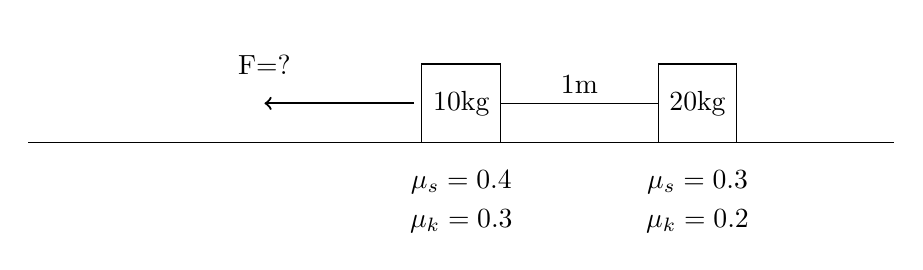
\begin{tikzpicture}
        \draw (0,0) rectangle (1,1) node[pos=.5] {10kg};
        \node at (0.5,-0.5) {$\mu_{s}=0.4$};
        \node at (0.5,-1.0) {$\mu_{k}=0.3$};
        \draw (3,0) rectangle (4,1) node[pos=.5] {20kg};
        \node at (3.5,-0.5) {$\mu_{s}=0.3$};
        \node at (3.5,-1.0) {$\mu_{k}=0.2$};

        \draw (1,0.5) -- (3,0.5) node[anchor=south,pos=.5] {1m};
        \draw [thick, ->] (-0.1,0.5) -- (-2,0.5) node[anchor=south, inner sep=10pt] {F=?};
        \draw (-5,0) -- (6,0);
    \end{tikzpicture}
    
\end{center}

\begin{parts}
    \part
    Draw a free body diagram for each block.

    \part
    What is the minimum force $F$ required?

    \part
    After the blocks start moving. What is the acceleration?

    \part
    What is the tension in the rope between the two blocks?

    \part
    Suddenly after 15 seconds, the police come and Mr. Stewart stops dead in his tracks. Although the silver block stops with him, the gold block continues forward. Using Newton's Laws, explain why this occurs.
    
    \part
    Will the gold block collide with the silver block? If so, what will its speed be when it collides?

    \part
    The bored 60kg police officer asks Mr. Stewart to drag the blocks back to the bank. However, he decides to sits on the gold block. Mr. Stewart agrees and starts dragging the blocks back. There is enough friction between the officer and the gold block such that he does not slide off. Draw a free body diagram for the silver block, the gold block, and the police officer when the system is moving. 

    \part
    When Mr. Stewart is moving at 1m/s, the police officer tells him to move at a constant velocity. What force does Mr. Stewart need to pull with to maintain a constant velocity of 1m/s?

    \part
    However, after doing what he is told, Mr. Stewart is getting rebellious. He decides to increase his velocity just enough so the police officer starts sliding off. If the coefficient of static friction between him and the gold block is $\mu_s=0.5$, how much does he need to increase the force he's currently applying?
\end{parts}

\question
Mr. Stewart is taken into custody. However, when no one was looking he ran into a small closet. He thought he was safe, but when he heard approaching footsteps he was forced to hide. Using his superhuman strength, he hid at the top of the closet wedged between two opposing walls. His hands and feet exert a force of $80N$ each on the walls, which is just enough to keep him still.

\begin{center}
    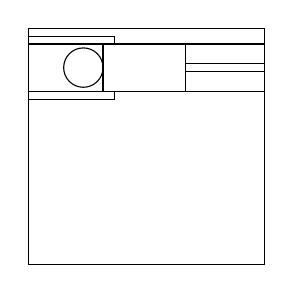
\begin{tikzpicture}
        \draw (0,0) rectangle (3,3);
        \draw (0,2.1) rectangle (1.1,2.2);
        \draw (0,2.9) rectangle (1.1,2.8);

        \draw (0.7,2.5) circle (0.25);

        \draw (0.95,2.8) rectangle (2,2.2);
        \draw (2,2.2) rectangle (3,2.45);
        \draw (2,2.8) rectangle (3,2.55);

    \end{tikzpicture}
\end{center}

\begin{parts}
    \part
    Draw a free body diagram for his hands (as one object) and his feet (as one object).
    \part
    What is the coefficient of static friction between the room and Mr. Stewart?
    \part
    Suddenly, a police officer walks in. Luckily, he does not see Mr. Stewart hiding. However, the room starts accelerating at $1m/s^2$ vertically. Mr. Stewart finds that he needs to exert more force to stay stationary relative to the elevator. Is the elevator moving up or down?
    \part
    What is the minimum force his hands and feet need to exert now?
\end{parts}

\question
After the officer leaves and escaping the elevator, Mr. Stewart finds himself on the roof of the police station. He spots a heavy block attached to a pulley with a long rope. Mr. Stewart decides to grab the end of the rope and descend, using the block to slow his descent. The building is 20 meters high and Mr. Stewart can survive the fall if he contacts the ground at $15 m/s$. The coefficient of kinetic friction between the block and the roof is $0.8$.

\begin{center}
    \begin{tikzpicture}
        \draw (0,0) rectangle (5,8);
        \draw (1,8) rectangle (2,9) node[pos=0.5] {$m=?$};
        \filldraw[fill=white, draw=black] (5,8) circle (0.5);

        \draw (2,8.5) -- (5,8.5);
        \draw (5.5,8) -- (5.5,4);

        \node at (1.5,7.5) {$\mu_{k}=0.8$};
        \node at (4,4) {$h=20m$};
    \end{tikzpicture}
\end{center}

\begin{parts}
    \part
    What is the minimum weight needed for the block in order for Mr. Stewart to live?
    \part
    5 meters down the building, the 60kg police officer from earlier comes and stands on the ramp. What is Mr. Stewart's acceleration?
    \part
    To try to slow down Mr. Stewart's descent even more, the police officer while still on the block, pushes down on the block with his hands with a force of $10N$. How much has Mr. Stewart's acceleration changed from part (b)?
    \part
    Will Mr. Stewart still be able to make it down safely? (Remember, Mr. Stewart can let go of the rope any time and live so long as the impact speed is less than $15 m/s$)
    \part
    Caught up in the heat of the motion, Mr. Stewart attempts to speed up his descent by pulling downwards on the rope he's attached to. Will this help? Use Newton's Laws to explain.
\end{parts}

\newpage
\question
As if it was a miracle, Mr. Stewart somehow survived and escaped the police station. He stumbles into an arid region, thirsty. Luckily, he finds a well. The well is 40m deep and he at the bottom there is a metal bucket of water. Luckily, there is a rope with one end attached to the bucket and another end at the surface. However, the rope seems in mad condition and can only withstand a maximum of 30N of force before it'll break. The bucket and water is approximately 2kg.

\begin{center}
    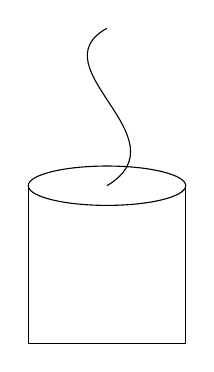
\begin{tikzpicture}
        \draw (0,0) ellipse (1 and 0.25);
        \draw (-1,0) -- (-1,-2) -- (1,-2) -- (1,0);
        \draw (0,0) .. controls (1,0.6) and (-0.9,1.5) .. (0,2);
    \end{tikzpicture}
\end{center}

\begin{parts}
    \part
    What is the shortest time possible for Mr. Stewart to get the water he wants without breaking the string?
    \part
    Mr. Stewart wants to lower the bucket and get some more water when he finds another identical rope. He attaches that rope to the bucket as well such that he will be pulling on the ends of two ropes simultaneously. How long will it take for him to get the water from the bottom to the top now?
    \part
    What if Mr. Stewart adds another rope? What about 4 ropes? 5? Can you find a generalized expression for the shortest possible time if $n$ ropes are attached to the bucket?
\end{parts}
\end{questions}